This section separates what the signals show from what the inferential stage decides. The first three readings are exploratory: they point to where frequency content appears to be lost, and that direction is not a result but what the Bayesian analysis of \autoref{sec:bayesResults} tests under the rules of \autoref{tab:bayesDecisions}.

\subsection{The frequency sweep}

Across the fifteen geometries, all drawn in \autoref{sec:appSweep}, the forecast rebuilds a pure tone at the right frequency only over the lower part of the analysed band, and even there with holes near some candidate sites; above it the rollout mostly returns slow content unrelated to the input, punctuated by isolated excursions, and the reading is least stable across starting phases exactly where it is worst. The linear probes do not follow that pattern: over most of the band the internal state still separates a tone from its neighbours, including at frequencies the forecast no longer places correctly, and where the band tasks weaken they do so over ranges of frequencies rather than at single candidate sites, while the local $f\pm1$\,Hz task remains stronger. \autoref{fig:rec16-16} shows both readings at the reference geometry. The common case is therefore a frequency that the representation retains and the output loses, an observation that gives the study its direction rather than a confirmation of structural aliasing or of the claims of \autoref{sec:agent}.

\begin{figure}[ht]
    \centering
    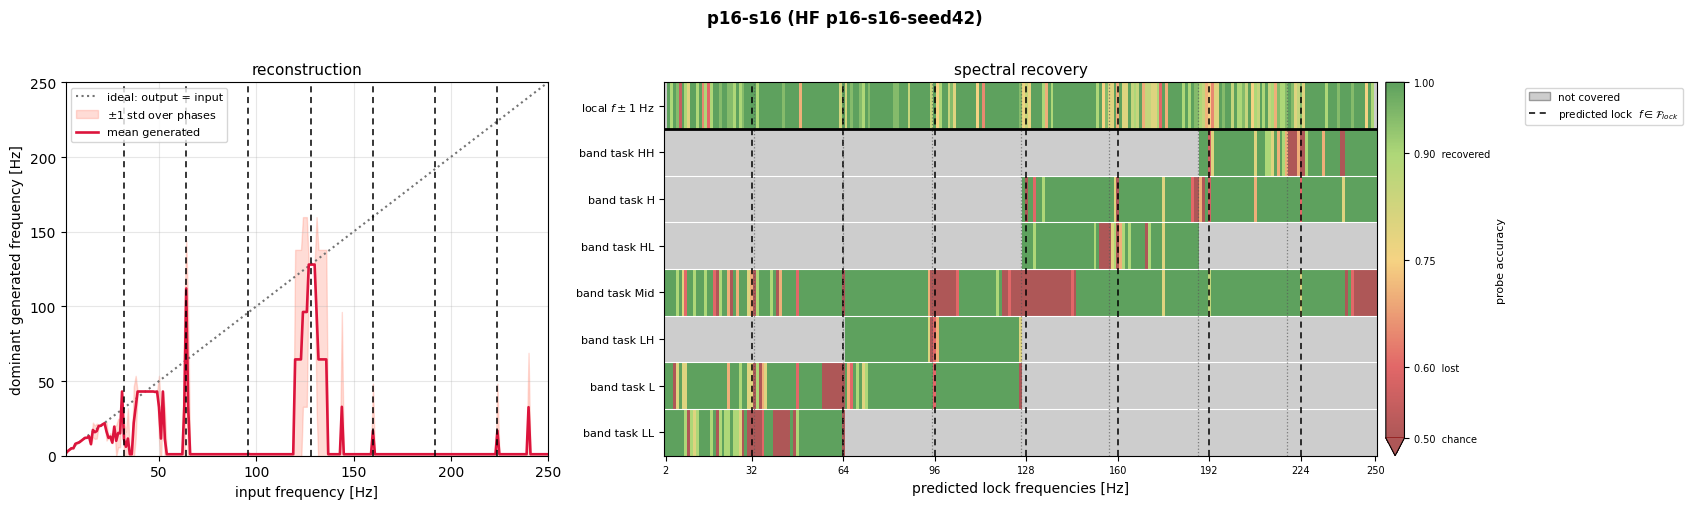
\includegraphics[width=\textwidth]{figures/fig_rec_16_16.png}
\caption{Behavioural reconstruction (left) and representational recovery (right) for pure tones under the retrained reference geometry $P=S=16$ and seed~42. The left panel compares input and dominant generated frequencies across phases; the right reports local and hierarchical band-probe accuracy. Dashed vertical lines mark the predicted lock frequencies, and grey cells denote frequencies outside a task's coverage.}
    \label{fig:rec16-16}
\end{figure}

\subsection{Recovering a component from a complex background}

When a single tone is added to a Light TSMixup or KernelSynth background, the retrained models seldom return it, and the exploratory analysis over a large sample of such draws gave a result that was not expected: the injected tone is much harder to intercept at the control frequencies than at the candidate sites, reappearing in about a quarter of the trials on a site and almost never beside one (\autoref{tab:decomposition}; procedure and single draws in \autoref{sec:appDecomp}). The pattern is the same for both generators, with the smallest patch retaining the most and the widest the least, which suggests that it belongs to the geometry rather than to the signal family, and the published checkpoint, which shares the reference geometry, returns added components more often on and off the sites. The result runs against the loss at the sites that $H1$ predicts and against what the pure-tone sweep suggested, and two mechanisms may contribute to it: a tone on a candidate site produces a repeating token sequence (\autoref{sec:tokenisation}) that a forecaster can prolong without representing the frequency, and the forecasts carry lines of their own on the candidate sites, which a count of presence credits as recovered. Whether a loss concentrates at the sites once background and phase are matched is what the Bayesian analysis decides.

\begin{table}[!t]
    \centering
    \small
    \begin{tabular}{@{}lrrrr@{}}
        \toprule
        \textbf{Generator} & \textbf{Components} & \textbf{Recovered} & \textbf{Missed} & \textbf{Displaced} \\
        \midrule
        Light TSMixup & --- & --- & --- & --- \\
        KernelSynth   & --- & --- & --- & --- \\
        \midrule
        \multicolumn{1}{@{}l}{\textbf{On $\mathcal F_{\mathrm{lock}}$}} & --- & --- & --- & --- \\
        \multicolumn{1}{@{}l}{\textbf{Off $\mathcal F_{\mathrm{lock}}$}} & --- & --- & --- & --- \\
        \bottomrule
    \end{tabular}
\caption{\textcolor{red}{\textbf{Placeholder table, to be filled from the decomposition notebook.} One row per generator and one per position relative to the candidate set, with the number of input components, how many are recovered from the forecast, how many are absent and how many return at a different frequency. The columns are indicative and will follow whatever the notebook reports.}}
    \label{tab:decomposition}
\end{table}


\subsection{Prediction on the measured series}

On the photovoltaic series every checkpoint forecasts the same windows spread across the year and is scored on the same minutes (\autoref{sec:appSolar}). The error is concentrated in daylight and in the transitions around sunrise and sunset, whereas at night almost every model correctly continues a series held at zero, and a typical forecast prolongs the level of the last hour while the measured power has already begun to change. The published checkpoint is the most accurate, again more plausibly because of its training than of its geometry; among the retrained models none improves on the $P=S=16$ baseline, several cannot be told apart from it and the rest are moderately worse, with no ordering by overlap or by patch size. One geometry, p32-s20, stands apart with a much larger error and non-zero output at night, which points to an issue with that checkpoint that still has to be verified.

The series offers insight into the application domain rather than a test of the design, because the dominant content of every window is the daily cycle, far below the first candidate site at one cycle per patch, so no window carries energy on $\mathcal F_{\mathrm{lock}}$. For the application the direction is nonetheless clear: content at the candidate sites reaches this plant only through weather transients lasting a few minutes, and those are the events a forecaster of this series would be least able to represent.

\FloatBarrier

\subsection{Bayesian analysis}\label{sec:bayesResults}

\textcolor{red}{\textbf{Placeholder of 600 words, to be replaced once the Bayesian fits are complete.} Report the posterior estimates of the models of \autoref{tab:bayesModels} with their credible intervals, the verdict of each rule of \autoref{tab:bayesDecisions} (supported, refuted or inconclusive), and the convergence diagnostics and posterior predictive checks that gate them. State, for each direction suggested by the readings above, whether the corresponding hypothesis is supported, refuted or left inconclusive. This is the only subsection in which a statement about the hypotheses is made; the readings above give the study its direction and are not used to decide any of them. Lorem ipsum dolor sit amet consectetur adipiscing elit sed do eiusmod tempor incididunt ut labore. Et dolore magna aliqua Ut enim ad minim veniam quis nostrud exercitation ullamco laboris nisi. Ut aliquip ex ea commodo consequat Duis aute irure dolor in reprehenderit in voluptate velit. Esse cillum dolore eu fugiat nulla pariatur Excepteur sint occaecat cupidatat non proident sunt in. Culpa qui officia deserunt mollit anim id est laborum Lorem ipsum dolor sit amet consectetur. Adipiscing elit sed do eiusmod tempor incididunt ut labore et dolore magna aliqua Ut enim. Ad minim veniam quis nostrud exercitation ullamco laboris nisi ut aliquip ex ea commodo consequat. Duis aute irure dolor in reprehenderit in voluptate velit esse cillum dolore eu fugiat nulla. Pariatur Excepteur sint occaecat cupidatat non proident sunt in culpa qui officia deserunt mollit anim. Id est laborum Lorem ipsum dolor sit amet consectetur adipiscing elit sed do eiusmod tempor. Incididunt ut labore et dolore magna aliqua Ut enim ad minim veniam quis nostrud exercitation. Ullamco laboris nisi ut aliquip ex ea commodo consequat Duis aute irure dolor in reprehenderit. In voluptate velit esse cillum dolore eu fugiat nulla pariatur Excepteur sint occaecat cupidatat non. Proident sunt in culpa qui officia deserunt mollit anim id est laborum Lorem ipsum dolor. Sit amet consectetur adipiscing elit sed do eiusmod tempor incididunt ut labore et dolore magna. Aliqua Ut enim ad minim veniam quis nostrud exercitation ullamco laboris nisi ut aliquip ex. Ea commodo consequat Duis aute irure dolor in reprehenderit in voluptate velit esse cillum dolore. Eu fugiat nulla pariatur Excepteur sint occaecat cupidatat non proident sunt in culpa qui officia. Deserunt mollit anim id est laborum Lorem ipsum dolor sit amet consectetur adipiscing elit sed. Do eiusmod tempor incididunt ut labore et dolore magna aliqua Ut enim ad minim veniam. Quis nostrud exercitation ullamco laboris nisi ut aliquip ex ea commodo consequat Duis aute irure. Dolor in reprehenderit in voluptate velit esse cillum dolore eu fugiat nulla pariatur Excepteur sint. Occaecat cupidatat non proident sunt in culpa qui officia deserunt mollit anim id est laborum. Lorem ipsum dolor sit amet consectetur adipiscing elit sed do eiusmod tempor incididunt ut labore. Et dolore magna aliqua Ut enim ad minim veniam quis nostrud exercitation ullamco laboris nisi. Ut aliquip ex ea commodo consequat Duis aute irure dolor in reprehenderit in voluptate velit. Esse cillum dolore eu fugiat nulla pariatur Excepteur sint occaecat cupidatat non proident sunt in. Culpa qui officia deserunt mollit anim id est laborum Lorem ipsum dolor sit amet consectetur. Adipiscing elit sed do eiusmod tempor incididunt ut labore et dolore magna aliqua Ut enim. Ad minim veniam quis nostrud exercitation ullamco laboris nisi ut aliquip ex ea commodo consequat. Duis aute irure dolor in reprehenderit in voluptate velit esse cillum dolore eu fugiat nulla. Pariatur Excepteur sint occaecat cupidatat non proident sunt in culpa qui officia deserunt mollit anim. Id est laborum Lorem ipsum dolor sit amet consectetur adipiscing elit sed do eiusmod tempor. Incididunt ut labore et.}
